\documentclass[10pt,twocolumn]{article}

\usepackage{url}
\usepackage{graphicx}
\usepackage{indentfirst}
\usepackage{titlesec}
\usepackage{geometry}
% \usepackage[showframe]{geometry}
\usepackage{layout}
\usepackage{lipsum}
\geometry{top=80pt, bottom=80pt}

\titlespacing*{\section}{0pt}{7pt}{4pt}
\titlespacing*{\subsection}{0pt}{5pt}{4pt}

\setlength{\headsep}{0pt}

\titleformat{\section}
  {\normalfont\scshape}{\thesection}{1em}{}

\titleformat{\subsection}
  {\normalfont\scshape}{\thesubsection}{1em}{}

\newenvironment{boldenv}
  {\bfseries}

\begin{document}

\title{Robust Lens Flare Removal}
\author{Floris Chabert}
\date{}
\maketitle

\begin{abstract}\begin{boldenv}
\lipsum[1]
\end{boldenv}\end{abstract}

\section{Motivation}

Lens flare and ghosting can be prevalent artifacts when taking pictures of a scene with a direct bright light (see Figure 1). Those artifacts are usually caused by internal reflections of the lens due to a thin anti reflective coating.

\indent
This project aims at automatically removing those lens artifacts to produce a clean image. We will design an algorithm involving two steps: flare detection and recovery of the damaged region.

\section{Related Work}

\lipsum[1]

\section{Method}

\begin{figure}[ht!]
\centering
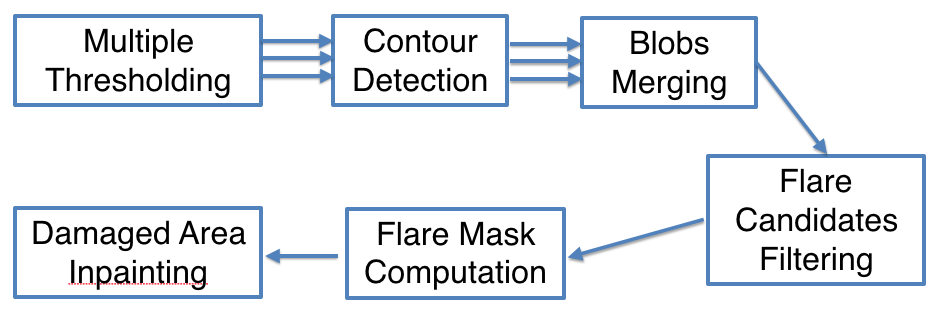
\includegraphics[width=72mm]{Flow.png}
\caption{Lens flare detection and restoration algorithm}
\end{figure}

\subsection{Detection}
The lens flare and ghosting will be precisely detected in the image. They have specific properties which can be used to segment the image [1].
Those can have different shapes and colors but the affected pixels usually saturate one or multiple color components of the image. We will first use thresholding and blob detection to segment the image and find the potential candidates. Then, other properties of those glares - their specific color and intensity distribution (halo shaped) - will allow us to eliminate potential false positive. We will evaluate the algorithm effectiveness with regard to the different categories of lens flare.

\begin{figure}[ht!]
\centering
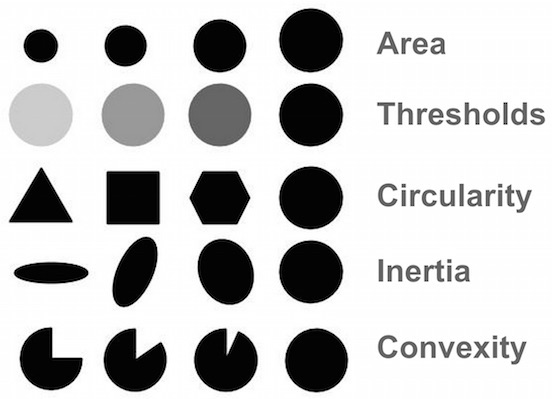
\includegraphics[width=72mm]{Filters.jpg}
\caption{Filtering parameters for blob detection[4]}
\end{figure}

\subsection{Recovery}
Finally, we will recover the area damaged by the identified artifacts. In order to fill those small regions we will use a partial differential equations inpainting algorithm based on the Curvature-Driven Diffusion model [2][3].

\section{Results}

\lipsum[1]

\begin{figure}[ht!]
\centering
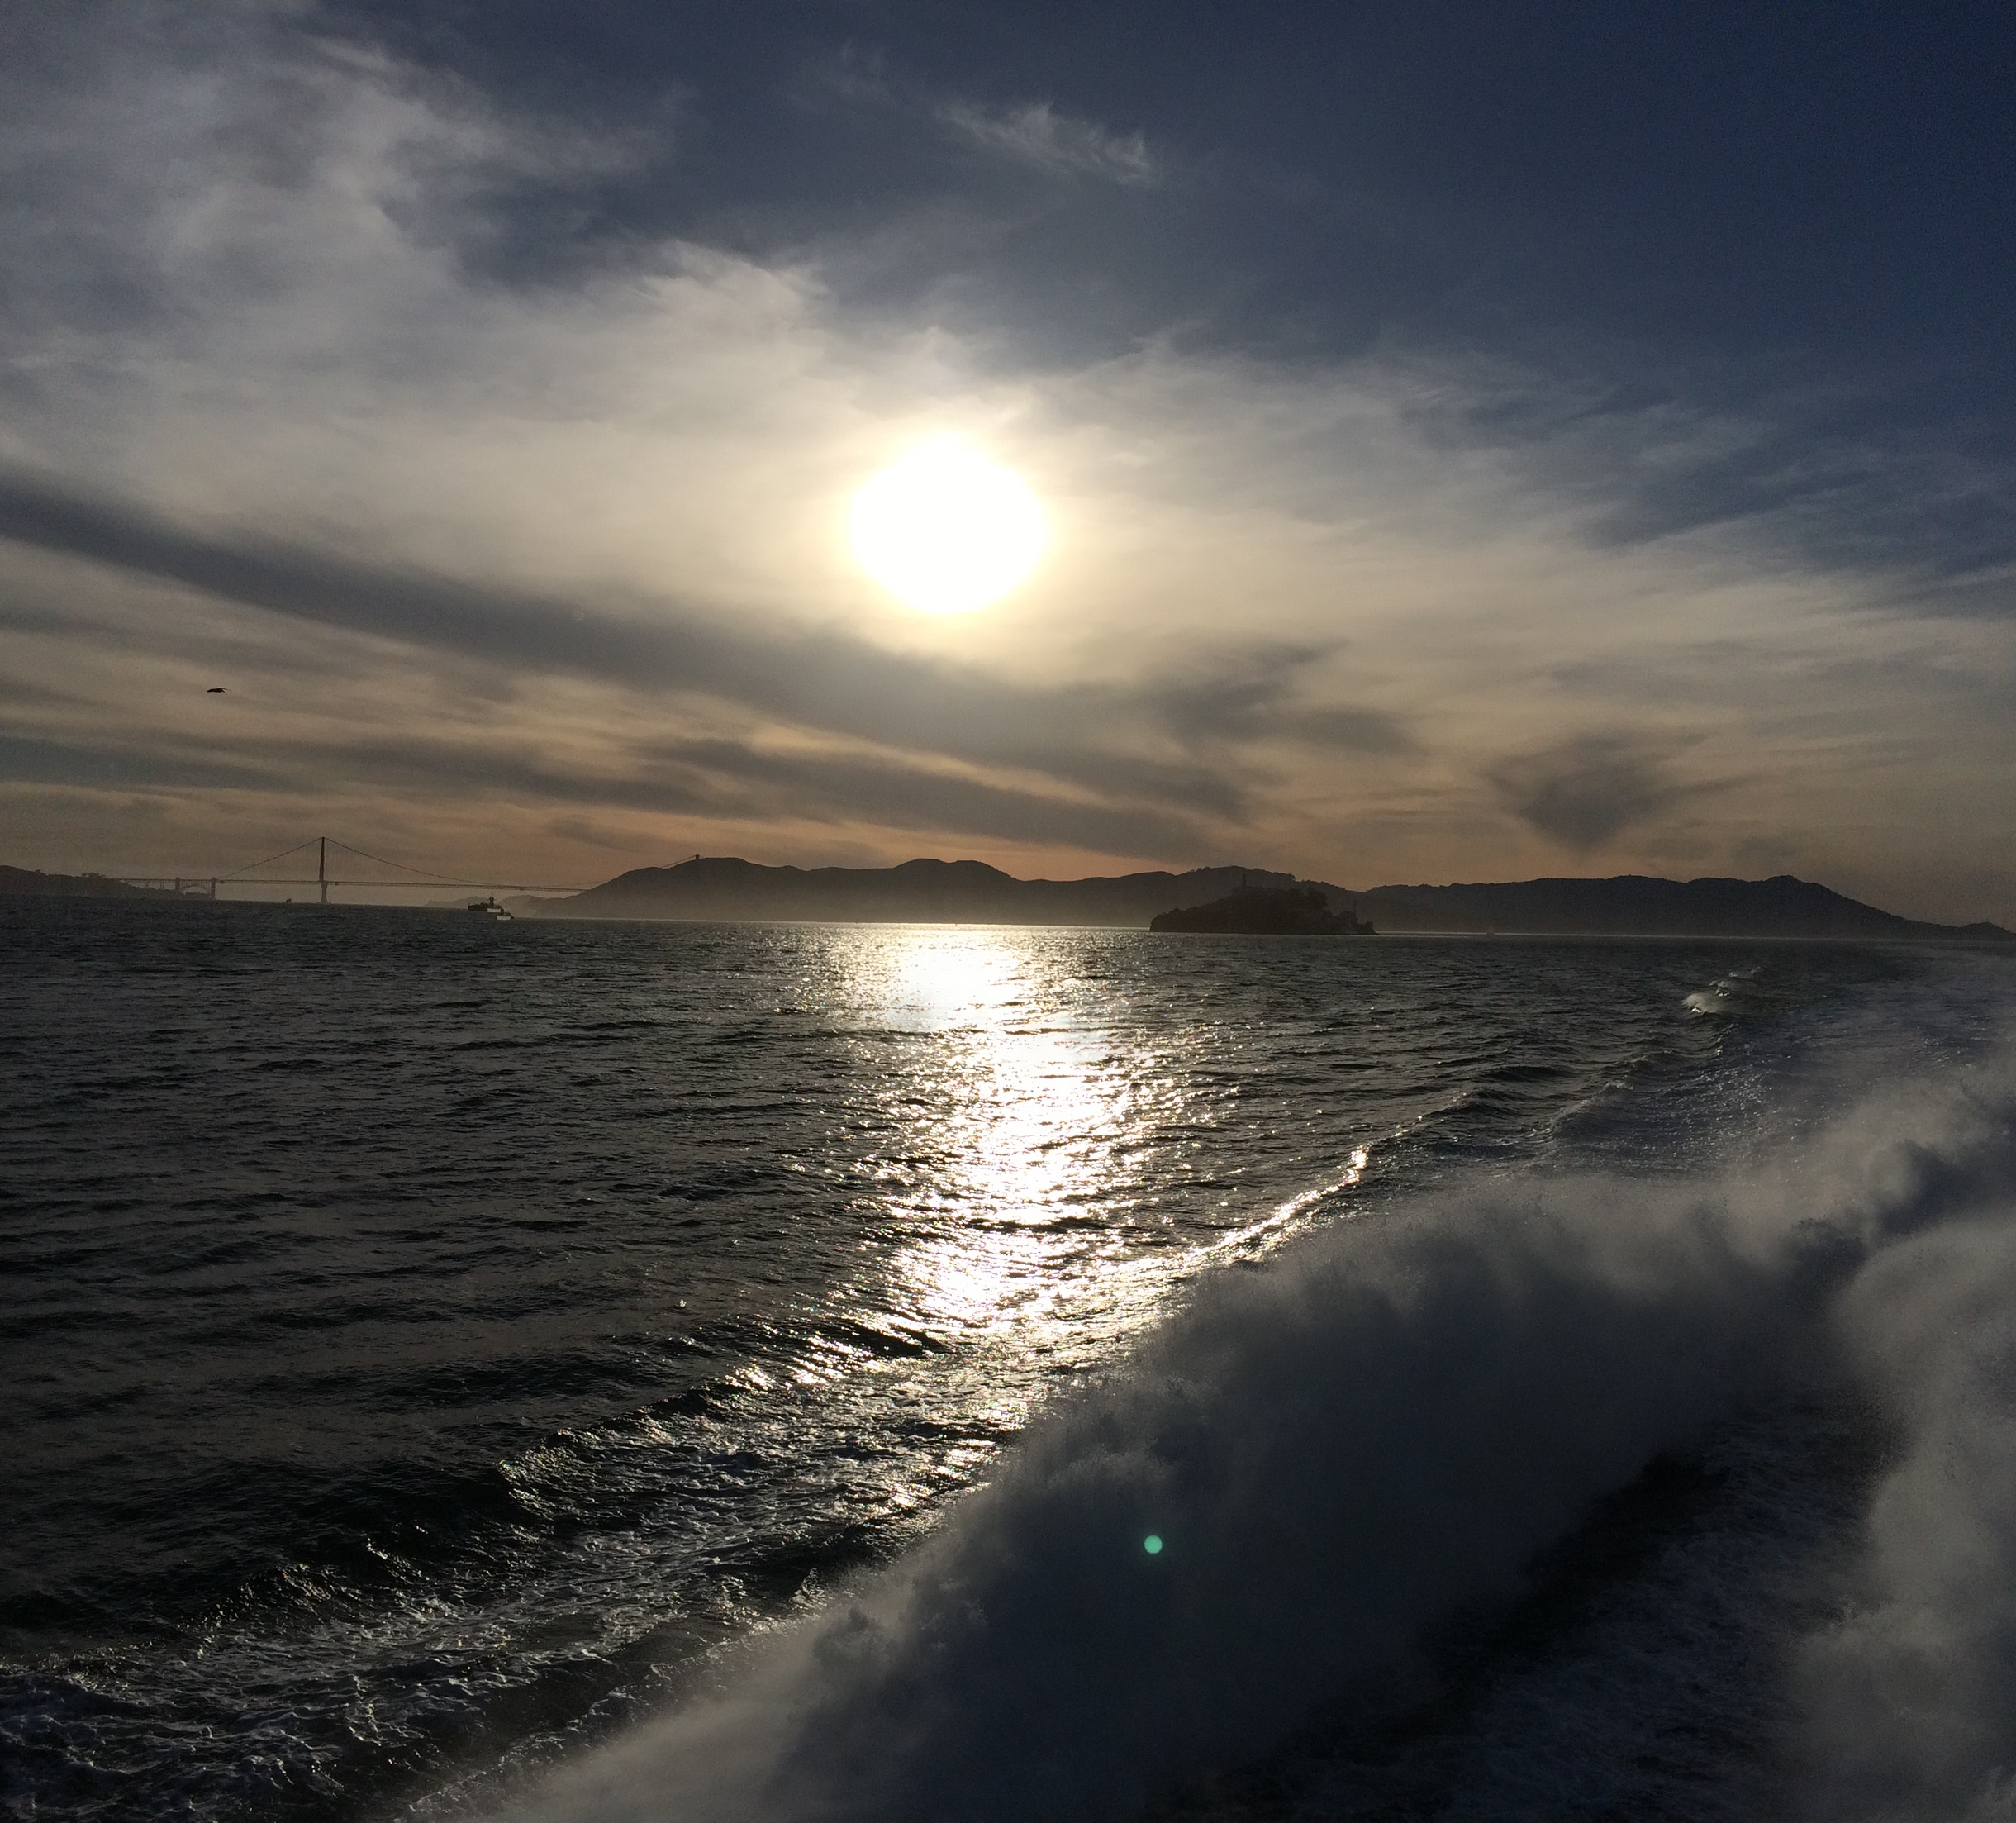
\includegraphics[width=72mm]{../Matlab/Images/1.jpg}
\caption{Pictures with lens flare artifact}
\end{figure}

\section{Discussion}

\lipsum[1]

\begin{thebibliography}{1}

\bibitem
Dusan Psotny,
\emph{Removing lens flare from digital photographs},
Charles University in Prague, Diploma Thesis

\bibitem
Andreas Nussberger, Helmut Grabner, Luc Van Gool,
\emph{Robust Aerial Object Tracking in Images with Lens Flare},
Comput. Vision Lab., ETH Zurich

\bibitem
Chil-Suk Cho, Joongseok Song, Jong-Il Park,
\emph{Glare Region Detection in Night Scene usig Multi-Layering},
Department of Electronics and Computer Engineering, Hanyang University

\bibitem
Aatya Mallick
\emph{Blob Detection Using OpenCV},
learnopencv.com

\bibitem
Tony F. Chan, Jianhong Shen
\emph{Mathematical Models for Local Nontexture Inpaintings}
SIAM Journal on Applied Mathematics, Vol. 62, No. 3

\bibitem
Tony F. Chan, Jianhong Shen,
\emph{Non-Texture Inpainting by Curvature-Driven-Diffusions},
Visual Comm Image Rep 06/2001

\bibitem
Jiansheng Liu, Mingming Li, Fangfang He
\emph{A Novel Inpainting Model for Partial Differential Equation Based on Curvature Function},
Journal of Multimedia, Vol. 7, No. 3, 2012

\end{thebibliography}

\end{document}